% Тут используется класс, установленный на сервере Papeeria. На случай, если
% текст понадобится редактировать где-то в другом месте, рядом лежит файл matmex-diploma-custom.cls
% который в момент своего создания был идентичен классу, установленному на сервере.
% Для того, чтобы им воспользоваться, замените matmex-diploma на matmex-diploma-custom
% Если вы работаете исключительно в Papeeria то мы настоятельно рекомендуем пользоваться
% классом matmex-diploma, поскольку он будет автоматически обновляться по мере внесения корректив
%

% По умолчанию используется шрифт 14 размера. Если нужен 12-й шрифт, уберите опцию [14pt]
\documentclass[14pt]{matmex-diploma}
%\documentclass[14pt]{matmex-diploma-custom}
\usepackage{listings}
\usepackage{subcaption}


\begin{document}
% Год, город, название университета и факультета предопределены,
% но можно и поменять.
% Если англоязычная титульная страница не нужна, то ее можно просто удалить.
\filltitle{ru}{
    chair              = {
Кафедра системного программирования
},
    title              = {Использование нейронных сетей для распознавания 16s РНК по вторичной структуре},
    % Здесь указывается тип работы. Возможные значения:
    %   coursework - Курсовая работа
    %   diploma - Диплом специалиста
    %   master - Диплом магистра
    %   bachelor - Диплом бакалавра
    type               = {coursework},
    position           = {студента},
    group              = 344,
    author             = {Лунина Полина Сергеевна},
    supervisorPosition = {к.\,ф.-м.\,н., доцент},
    supervisor         = {Григорьев С.\,В.},
%   university         = {Санкт-Петербургский Государственный Университет},
%   faculty            = {Математико-механический факультет},
%   city               = {Санкт-Петербург},
%   year               = {2013}
}
\maketitle
\tableofcontents
% У введения нет номера главы
\section*{Введение}
Биоинформатика включает в себя ряд задач, решения которых необходимы в биологических исследованиях. Одной из часто встречающихся в биоинформатике задач является задача классификации микроорганизмов, которая проводится на основе генетических данных, находящихся в полученных из окружающей среды образцах. В любом геноме присутствуют определенные участки --- маркерные последовательности, --- позволяющие однозначно определить вид данного организма, а также обнаружить структурное сходство организмов и предположить, например, наличие у них общего предка. Существуют базы данных последовательностей РНК, используемые для создания и тестирования различных алгоритмов классификации, например, SILVA \cite{5} или The Greengenes Database \cite{14}.

Для идентификации и таксономической классификации бактерий обычно исследуется ген 16s РНК. В геноме любого прокариотического организма (организма, не имеющего оформленного ядра) присутствует, по меньшей мере, одна копия этого гена \cite{1}. Молекула 16s РНК, как и  любой другой РНК, состоит из одной полинуклеотидной цепи, отдельные участки которой соединяются между собой, образуя сложную и стабильную вторичную структуру. В задачах классификации часто анализируется последовательность нуклеотидов в первичной структуре 16s РНК, как, например, в классификаторе, описанном в работе \cite{2}. 

При сравнении первичных структур 16s РНК различных организмов было обнаружено, что некоторые их участки (консервативные) одинаковы для всех видов, другие же (гипервариабельные) могут в разной степени различаться \cite{3}, что позволяет в задачах классификации рассматривать только часть последовательности нуклеотидов. Тем не менее, исследования показывают, что рассмотрение не только первичной, но и вторичной структуры молекулы РНК может дать более точный результат, так как вторичная структура не менее информативна и может содержать в себе достаточную для классификации информацию \cite{4}.

Данные о вторичной структуре молекулы могут быть получены с помощью различных технологий. В последнее время в биоинформатике получили широкое распространение инструменты синтаксического анализа, в терминах которого РНК представляет из себя последовательность символов в алфавите \{A, C, G, U\}, а правила образования вторичной структуры для каждого отдельного вида можно задать некоторой грамматикой. Для работы с такими грамматиками существуют специальные алгоритмы, например, платформа YaccConstructor \cite{15}. Таким образом, обработав последовательность нуклеотидов, являющуюся 16s или же другим участком генома, с помощью заданной грамматики, можно получить некоторую информацию о вторичной структуре, которая затем может быть представлена в пригодном для изучения виде, например, в виде изображения, вектора, графа и др. 

В качестве метода исследования в задачах распознавания и классификации иногда используется машинное обучение, так как распознавание маркерных генов с помощью точных методов часто затруднено присутствием различных мутаций, “шумов” и других неточностей в полученных из окружающей среды образцах. Кроме того, во входных данных могут также встречаться геномы не известных ранее организмов. Из-за этого использование точных алгоритмов в некоторых случаях может оказаться недостаточно продуктивным, в то время как такой метод, как машинное обучение, направленный на выявление более общих закономерностей, может работать с лучшей точностью. 

Предполагается, что молекулы 16s РНК обладают достаточно характерной вторичной структурой, и поэтому полученные с помощью синтаксического анализа данные могут быть применимы для распознавания и классификации методами машинного обучения. Для проверки этой гипотезы в данной работе была создана нейронная сеть, распознающая последовательности 16s РНК, обработанные методами синтаксического анализа, среди прочих нуклеотидных последовательностей.

\section{Цель и задачи}
Цель данной работы --- исследование возможности распознавания бактерий на основе данных о вторичной структуре их 16s РНК, полученных методами синтаксического анализа, с помощью машинного обучения.
Для достижения цели были поставлены следующие задачи:
\begin{itemize}
    \item разработка архитектуры решения;
    \item выбор формата представления данных о вторичной структуре и реализация процесса их генерации;
    \item создание нейронной сети для распознавания 16s РНК среди прочих нуклеотидных последовательностей;
    \item экспериментальные исследования и анализ полученных результатов.
\end{itemize}

\section{Обзор}
\subsection{Существующие решения в области распознавания и классификации организмов}
Последовательность нуклеотидов может быть рассмотрена как текст, обладающий некоторыми синтаксическими особенностями, которые, с биологической точки зрения, задают вторичную структуру молекулы РНК. Существуют различные подходы к исследованию закономерностей образования вторичной структуры с точки зрения синтаксического анализа, например, стохастические контекстно-свободные грамматики \cite{10} или формальные грамматики, включающие псевдоузлы \cite{11}.

Рассмотрение вторичной структуры играет существенную роль в задачах классификации, так как последовательность нуклеотидов первичной структуры не всегда является универсальным критерием для идентификации организма, в то время как данные о вторичной, являющейся более консервативной, могут отразить некоторые необходимые для классификации особенности \cite{12}.

Существуют инструменты  для распознавания и классификации организмов, использующие наряду с первичной структурой также и информацию о вторичной. Далее будут рассмотрены некоторые из них.

BLAST (Basic Local Alignment Search Tool) \cite{6} --- семейство программ для поиска гомологов белков и нуклеиновых кислот на основе их первичных структур. Для изучаемой последовательности и каждой последовательности из базы данных вычисляется, насколько они сходны. 

Многие участки нуклеотидных последовательностей 16s РНК схожи у родственных организмов, что позволяет достаточно широко применять метод сравнения первичных структур, однако в ряде случаев можно наблюдать сходство во вторичной структуре при несовпадении первичной.

В лаборатории Eddy/Rivas Laboratory \cite{7} разрабатываются методы анализа геномных последовательностей, учитывающие вторичную структуру: HMMER \cite{8} и Infernal \cite{9}.

Infernal (inference of RNA alignments) --- инструмент, который осуществляет поиск гомологов микроорганизма по данным о его РНК. Использует вероятностные модели (covariance models), работающие на основе стохастических контекстно-свободных грамматик.

HMMER --- инструмент для поиска гомологов и выравнивания последовательностей. В основе работы алгоритма лежит теория скрытых марковских моделей, с использованием которых моделируется вторичная структура. В отличие от Infernal, используется в основном для работы с белками и работает быстрее, но менее точно \cite{13}.

Кроме того, существуют решения задачи классификации, основанные на использовании нейронных сетей. Например, Humidor \cite{17} --- модель для классификации генетических данных об организмах с помощью сверточных нейронных сетей. Данные представлены в формате CIGAR strings, который позволяет описывать вставки, удаления и несоответствия входной последовательности относительно некоторой обобщающей последовательности (consensus sequence).

\subsection{Используемые технологии}
YaccConstructor \cite{15} --- исследовательский проект, созданный на кафедре системного программирования СПбГУ в лаборатории языковых инструментов JetBrains. В рамках данного проекта разрабатывается платформа для создания алгоритмов синтаксического анализа, реализованная на языке программирования F\#. 

Keras \cite{16} --- открытая библиотека для конструирования и обучения нейронных сетей, написанная на языке Python. Представляет собой надстройку над фреймворками Deeplearning4j, TensorFlow и Theano.

\section{Архитектура решения}
В данной работе была проверена возможность применения инструментов синтаксического анализа для исследования вторичных структур геномных последовательностей.

Структуру решения можно разделить на две смысловые части: подготовка входных данных и их анализ с помощью нейронной сети (Рис.~\ref{1}).

\begin{figure}[!ht]
\centering
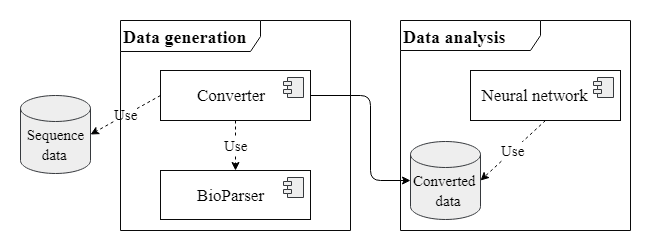
\includegraphics[width=15cm]{architecture.png}
\caption{Архитектура решения}
\label{1}
\end{figure}

Первоначальные входные данные --- база данных нуклеотидных последовательностей, поделенных на два класса: 16s РНК бактерий из базы данных SILVA и случайные последовательности, вырезанные из полных геномов бактерий.

Далее на базе платформы YaccConstructor был реализован процесс генерации данных, хранящих информацию о вторичной структуре. Для этого нуклеотидные последовательности были обработаны с помощью выбранного алгоритма синтаксического анализа по некоторой зафиксированной грамматике. Затем полученные структуры данных были преобразованы в подходящий для обучения нейронной сети формат.


Полученная таким образом новая база данных была изучена с помощью нейронной сети, реализованной на базе библиотеки Keras и фреймворка TensorFlow. Нейронная сеть осуществляет бинарную классификацию, т.е. определяет для тестируемого образца его принадлежность к классу 16s РНК.


\section{Выбор формата данных и реализация процесса их генерации}
Одной из задач данной работы являлся выбор формата представления данных о вторичной структуре микроорганизмов, полученных с помощью синтаксического анализа, и реализация процесса их генерации. 


Для обработки берется последовательность нуклеотидов, состоящая из символов алфавита \{A, C, G, U\}, т.е. первичная структура. Вторичная структура --- это спсоб укладки полинуклеотидной цепи в более компактную структуру (Рис.~\ref{2}). Изучение вторичных структур различных 16s РНК позволяет обнаружить наличие некоторых закономерностей в этом способе укладки. 

\begin{figure}[!ht]
\centering
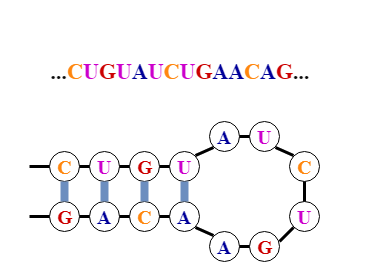
\includegraphics[width=10cm]{structures.png}
\caption{Первичная и вторичная структуры РНК}
\label{2}
\end{figure}

Эти закономерности зависят от наличия в геномной последовательности подпоследовательностей определенного вида. Таким образом, нужен способ показать для цепочки символов, присутствуют ли в ней подцепочки, которые при свертке позволят идентифицировать ее как молекулу 16s РНК какого-либо организма и в идеале определить видовую принадлежность.


Закономерности свертки строки в терминах синтаксического анализа могут быть заданы с помощью грамматики. Поэтому необходимо найти оптимальную для решения поставленной задачи грамматику.


В данной работе построение грамматики было основано на следующих соображениях. В результате синтаксического анализа должны быть извлечены особенности вторичной структуры, достаточные для решения поставленных задач, и выбранная грамматика должна описывать эти особенности. При этом необходимо, чтобы она минимально учитывала первичную структуру, т.е не содержала перечислений консервативных первичных последовательностей. Основная особенность, доступная для описания в терминах контекстно-свободной грамматики --- шпилька и композиции шпилек (Рис.~\ref{3}). Шпилька --- элемент вторичной структуры, который образуется, когда две последовательности одной и той же цепи комплементарны друг другу и соединяются друг с другом, образуя на конце неспаренный участок --- петлю.



\begin{figure}[!ht]
    \centering
    \begin{subfigure}[b]{0.4\textwidth}
\begin{verbatim}
[<Start>] 
s1: stem<s0> 
s0: A U C U G A 
stem<s>: 
     A s U 
    | G s C 
    | U s A 
    | C s G
\end{verbatim}
    \end{subfigure}
\begin{subfigure}[b]{0.4\textwidth}
        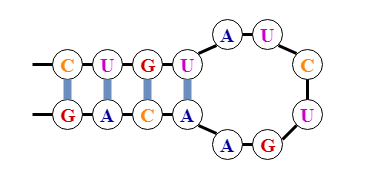
\includegraphics[width=8cm]{grammar.png}
    \end{subfigure}
\caption{Пример задания шпильки с помощью грамматики}
\label{3}
\end{figure}


При построении грамматики нужно учитывать, что, чем больше минимальная высота шпильки, тем реже она будет встречаться, т.е. при задании слишком большой минимальной высоты может оказаться, что таких шпилек не существует в цепочке. Тогда грамматика не будет выявлять характерные особенности вторичной структуры. С другой стороны, нужно отразить в грамматике тот факт, что между шпильками могут присутствовать участки, которые не стягиваются в шпильку. При слишком большой верхней границе на длину такого участка вся цепочка может не содержать шпилек, а при слишком маленькой между шпильками окажутся пропуски. В этих случаях грамматика также окажется бесполезной. На данный момент грамматика построена на основе вышеизложенных соображений и визуального изучения вторичных структур 16s РНК из различных работ (Рис.~\ref{4}).



\hfill
\begin{figure}[ht!]
\begin{center}
\begin{verbatim}
[<Start>]
s1: stem<s0> any
a_0_7 : any*[2..10]
s0: a_0_7 | a_0_7 stem<s0> s0
any: A | U | C | G
stem1<s>: 
     A s U 
    | G s C 
    | U s A 
    | C s G
stem2<s>: stem1<stem1<s>>
stem<s>: 
      A stem<s> U
    | U stem<s> A
    | C stem<s> G
    | G stem<s> C
    | stem1<stem2<s>>
\end{verbatim}
\caption{КС-грамматика вторичной структуры 16s РНК}
\label{4}
\end{center}
\end{figure}


Кроме того, необходимо выбрать оптимальную длину входной строки, так как слишком короткая подпоследовательность последовательности нуклеотидов молекулы не будет включать в себя большую часть наиболее характерных шпилек, а слишком длинная потребует много времени на генерацию данных и обучение нейронной сети.

Таким образом, с учетом этих предположений были получены цепочки нуклеотидов длины 512 символов и контекстно-свободная грамматика, позволяющая выделить основные особенности, характерные для вторичной структуры. Далее по этим данным необходимо получить более конкретные структуры, пригодные для дальнейшей обработки. Для генерации входных данных были использованы алгоритмы синтаксического анализа, реализованные на базе платформы YaccConstructor.


Для разбора строки символов с помощью контекстно-свободной грамматики в данной работе был применен вариант алгоритма Вэлианта \cite{18}, который для входной строки длины n строит матрицу размера n$\times$n. хранящую информацию о выводимости данной строки в грамматике. Элементами данной матрицы являются множества нетерминальных символов грамматики. Эту матрицу можно представить в более удобном для решения конкретной задачи виде. В данной работе был зафиксирован один из нетерминалов (стартовый) и каждый элемент матрицы был заменен на 0 или 1 в зависимости от существования стартового среди множества нетерминалов в ячейке. Затем эта бинарная матрица была построчно преобразована в числовой вектор. Такой вектор в достаточно сжатом виде хранит результат работы синтаксического анализатора по входной строке и описанной выше грамматике.

Таким образом, результатом работы реализованного алгоритма генерации данных является база данных числовых векторов, для каждого из которых известно, получен он из последовательности 16s РНК какой-либо бактерии или же из другого участка генома.


\section{Создание нейронной сети}
Для обучения нейронной сети были подготовлены два набора данных: положительные, т.е. полученные из последовательностей 16s РНК различных бактерий и отрицательные, т.е. полученные из некоторых других случайных участков геномов. 

В качестве используемых технологий были выбраны фреймворк \linebreak TensorFlow и библиотека Keras, написанная на языке Python. Реализованная в данной работе нейронная сеть осуществляет бинарную классификацию числовых векторов, т.е. для каждого образца определяет, получен он из 16s РНК какого-либо организма или нет.

Выбор архитектуры нейронной сети был основан на следующих особенностях входных данных. Во-первых, они линейны, следовательно, для работы с ними лучше всего подходят обычные полносвязные слои (Dense layers). Во-вторых, данные достаточно сильно сжаты, и поэтому необходимо детально изучать даже небольшие их участки. Для этого были использованы Dropout слои, случайным образом отсеивающие некоторый процент элементов входного вектора перед каждым Dense слоем. В-третьих, большая длина входного вектора требует многослойности нейронной сети. Таким образом, была сконструирована модель, состоящая из 16 чередующихся Dense и Dropout слоев с Dropout процентом, варьирующимся от 0.5 до 0.75. Предполагается, что выбранная модель позволит, рассматривая более близко небольшие части входного вектора, определить наличие в нем характерных для вторичной структуры особенностей и подобрать веса для их корректного распознавания по всей длине. В качестве алгоритма оптимизации был выбран Adagrad (adaptive gradient), позволяющий выделить редко встречающиеся особенности входных данных, которые, тем не менее, могут оказаться достаточно информативными для задачи распознавания.

Для обучения, валидации и тестирования нейронной сети было взято 35706 векторов, поделенных в соотношении 50:20:30 соответственно. В ходе обучения была получена точность 0.89, точность на валидации составила 0.90.

\section{Эксперименты и анализ результатов}

В качестве тестовых данных было взято 7345 образцов, из которых половина являлась результатом обработки 16s РНК какого-либо организма. Были получены следующие результаты.
\begin{table}[h]
\begin{center}
  \begin{tabular}{ | c | c | c |}
    \hline
    & classified as positive & classified as negative \\
    \hline
    positive & TP = 2789 & FP = 856 \\
    \hline
    negative & FN = 108 & TN = 3592 \\
    \hline
  \end{tabular}
\end{center}
\caption{TP --- true positive, TN --- true negative, FP --- false positive, FN --- false negative }
\label{mistakes}
\end{table}

Для оценки качества работы модели были использованы стандартные метрики, основанные на вышеприведенных результатах бинарной классификации.
\begin{itemize}
    \item Accuracy = $\frac{TP+NT}{TP+TN+FP+FN}$ = 0.87
    \item Precision = $\frac{TP}{TP+FP}$ = 0.96
    \item Recall = $\frac{TP}{TP+FN}$ = 0.77
    \item Specificity = $\frac{TN}{TN+FP}$ = 0.97
\end{itemize}


Экспериментальные исследования показали, что обученная нейронная сеть распознает 16s РНК среди нуклеотидных последовательностей с достаточно высокой точностью, чтобы предположить, что гипотеза о существовании характерных особенностей образования вторичной структуры имеет право на существование. Таким образом, полученные из цепочек нуклеотидов с помощью методов синтаксического анализа данные содержат информацию, необходимую для определения их принадлежности к множеству 16s РНК различных организмов и пригодны для дальнейших исследований.


\section{Результаты}
В ходе данной работы с помощью машинного обучения были исследованы возможности распознавания бактерий на основе полученных с помощью алгоритмов синтаксического анализа данных о вторичной структуре их 16s РНК. Были получены следующие результаты:
\begin{itemize}
    \item разработана архитектура решения для проверки гипотезы;
    \item реализован процесс генерации данных в виде числовых векторов;
    \item создана нейронная сеть для распознавания 16s РНК бактерий среди прочих нуклеотидных последовательностей по данным о вторичной структуре;
    \item проведены экспериментальные исследования на участках геномов
    бактерий из базы данных SILVA.
\end{itemize}

Существует несколько направлений дальнейшего развития полученных результатов. Во-первых, эксперименты в области аннотации генома, т.е. определение местонахождения 16s РНК в полноразмерном геноме. Для этого необходимо научиться работать со строками, где подстроки нуклеотидов, относящиеся к 16s РНК расположены со сдвигом относительно начала или конца строки. Во-вторых, реализация модели нейронной сети для определения видовой принадлежности организма. В-третьих, оптимизация грамматики, описывающей вторичную структуру.

\setmonofont[Mapping=tex-text]{CMU Typewriter Text}
\bibliographystyle{ugost2008ls}
\bibliography{coursework.bib}
\end{document}
